{
\setlength{\parindent}{2em}
\chapter{State of the art}\label{cha:state-of-the-art}
Saving the state of a running application to a file has been a very well-known challenge in the world of computer science, one that has its roots back to when the computers became powerful enough to run complicated programs. With the rise of local networks and the Ethernet protocol in the 1970s, an increasing amount of processing units could be linked together through a local network in order to improve the execution speed of difficult computation \cite{book:andrews}. This gave rise to the field of distributed computing, where scalability, parallelization of algorithms and efficient inter-node communication are among the very active topics of research.

Of course, the more complicated a system is, the more failure-prone it becomes. This is why it's imperative for designers of such parallel algorithms to be careful when programming an application. The application has to be made in such a way that it stays tolerant to eventual faults in the computing nodes of the network. For instance, one can think of the algorithms involved in numerical weather prediction software, that theoretically never finish as long as updated data is fed into the system. It is important for the forecasting industry not to loose any of the results that were previously solved if an unfortunate event occurs. \textit{Fault-tolerant computing} is the research field that finds solutions to this problem in multiple ways. In the context of distributed computing, one of the ways to mitigate the problem is to use a checkpoint and restart mechanism.

This technique allows the program to save itself while its running, and to restart at a previous checkpoint if processing stops. A "save" can take many forms, and really, its content is ultimately decided by the makers of the program. The final design is driven by factors that need to be clarified beforehand :
\begin{enumerate}
	\item \textbf{What needs to be saved?} There needs to be a clear understanding of the program and how it works. Is saving only the intermediate result of a computation considered a sufficient condition to be able to restore the program back to where it was? Do we have to save the entire state of the operating system? Of the entire computer? 
	\item \textbf{What are we saving?} This can be binary data, numerical data, text, etc. This is again highly dependent on the application.
	\item \textbf{How are we saving it?} How can a checkpoint take form? This depends on the content. Most of the time, this will be a file written to non-volatile memory. Nevertheless, a suitable file format has to be used depending on the data.
	\item \textbf{How often do we need to save?} A checkpoint can take a lot of space, and that amount usually grows linearly with the number of execution threads. In huge systems, this is not a trivial question. In addition, not only does a checkpoint take up hard disk space, it also induces an overhead in the execution of the program. Depending on the desired granularity, saving the relevant data can take a significant amount of time. This is represented by $O_F$ in \autoref{fig:chkpt-scheme}. This factor is important, especially in big distributed systems where computing time is expensive. As an example, the Titan supercomputer in the United States racks up \$9 million USD in electricity bills yearly \cite{online:henn}.
	\item \textbf{How long does it take to restart?} Saving at checkpoints takes time, but so does recovery. \autoref{fig:chkpt-scheme} shows this with $R_F$. Another point to consider is how often we need to restart back. In the end, restarting to a past state must be as straightforward as possible.
\end{enumerate}
\begin{figure}[H]
	\centering
	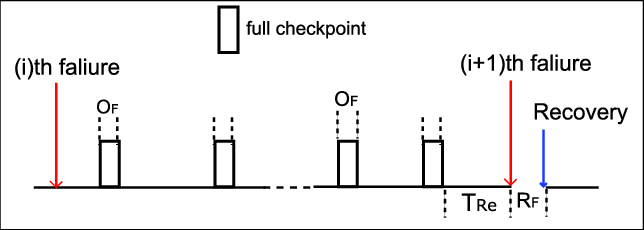
\includegraphics[width=0.9\linewidth, keepaspectratio]{art/checkpoint-scheme.png}
	\caption{Checkpoint/restart as a stochastic renewal reward process.}
	\label{fig:chkpt-scheme}
	\source{\textit{High Performance Computing Systems with Various Checkpointing Schemes} \cite{misc:chkpt-scheme}}
\end{figure}

\subsection*{Checkpointing schemes}
There are different checkpointing schemes that are adapted to different needs. On one hand, it is possible to checkpoint the application at predetermined intervals $\Delta t$ (i.e every minute). This can be useful in certain cases where it's applicable, because it puts an upper bound on the amount of data loss in a worst case scenario. However, this mitigation method is not always possible for every type of computation. 

The second approach is to do it sporadically. This can be used when it's impossible to predict the amount of time required for a computation. Unfortunately, it also means that the user doesn't know exactly when checkpoints will occur nor can he upper-bound the maximum amount of data/time loss.

 or sporadically, , automatically or with human intervention.

 and they are not only restricted to distributed systems. 

.

Why exactly can these concepts be useful in the case of a simulator? The checkpoint and restart technique is not only applicable to the distributed computing 
  
\section{Checkpoint and Restore in Userspace}\label{sec:criu}
\section{Berkeley Lab Checkpoint/Restart for Linux}\label{sec:blcr}

}